	El proyecto sTGC Mineria se compone de tres sistemas: disparo, detección y adquisición, como se ilustra en la Figura \ref{fig:sistema-completo}. El sistema de disparo \cite{Oyanadel2020SISTEMASTGC} ilustrado en azul, como se introdujo en la sección \ref{sec:planteamiento}, está constituido por dos detectores centelladores y una unidad de coincidencias que emite una señal digital de disparo (indicada en celeste) cuando un muón traspasa ambos detectores centelladores. Esta señal de disparo es necesaria para discriminar eventos captados por el detector sTGC y descartar interacciones procedentes de otras partículas cargadas que no sean muones.
	
	Si bien los detectores centelladores presentes en el sistema de disparo son capaces de detectar exclusivamente el paso de muones, en esta configuración experimental no son capaces de determinar la ubicación del vértice de interacción. Es por eso que son detectores complementarios al sistema de detección sTGC (ilustrado en verde en la Figura \ref{fig:sistema-completo}), sistema que es capaz de determinar la ubicación de los vértices de interacción gracias a su tecnología de fabricación.
	
	En este capítulo se detalla la forma y funcionamiento del sistema de detección, describiendo el prototipo de detector sTGC utilizado en sTGC Minería y describiendo también la interfaz de lectura ASD que lo sucede. Es necesario conocer las características de estas etapas, ya que determinan la cantidad y tipos de señales a leer en el sistema de adquisición de datos a ser diseñado en este proyecto de titulación.
	
	\begin{figure}[h]
		\centering
		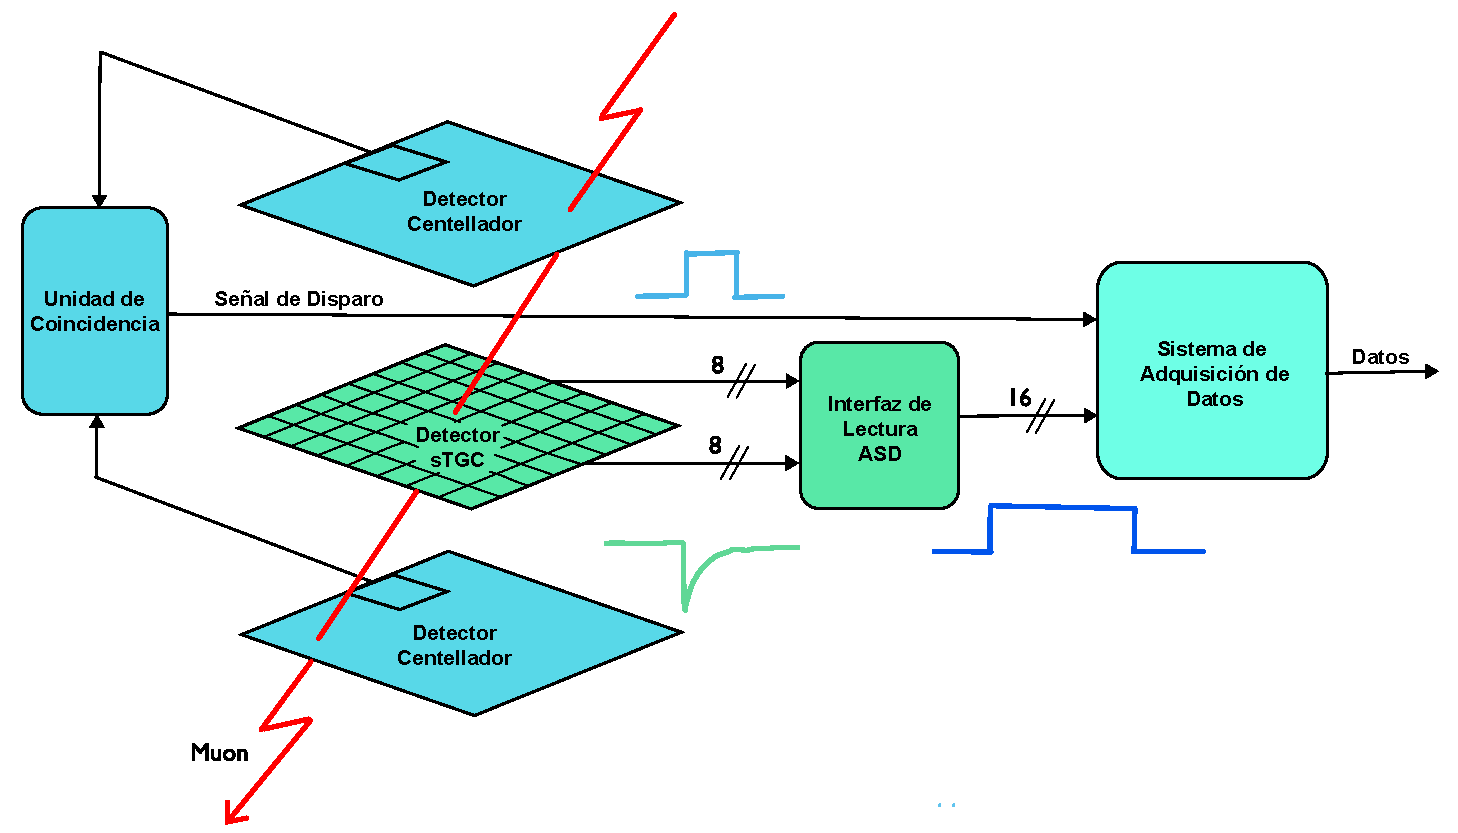
\includegraphics[scale=0.55]{sistema.pdf}
		\caption{Diagrama del sistema de muongrafía de terreno utilizando un solo detector.}
		\label{fig:sistema-completo}
	\end{figure}